
\documentclass[12pt,reqno]{book}      % Sets 12pt font, equation numbers on right
\usepackage{amsmath,amssymb,amsthm,amsfonts} % Typical maths resource packages
\usepackage{graphics}                 % Packages to allow inclusion of graphics
\usepackage{color}                    % For creating coloured text and background
\usepackage[margin=1in]{geometry}

\usepackage[colorlinks,citecolor=blue,linkcolor=blue]{hyperref}                 % For creating hyperlinks in cross references. It should be after the color package. The option colorlinks produces colored entries without boxes. The option citecolor=blue changes the default green citations to blue.

\usepackage{pgfplots}
\usepackage[mathscr]{euscript}
\usepackage{xcolor}
\usepackage{minted}

\DeclareGraphicsExtensions{.pdf}

\newtheorem{theorem}{Theorem}[section]
\newtheorem{proposition}[theorem]{Proposition}
\newtheorem{corollary}[theorem]{Corollary}
\newtheorem{lemma}[theorem]{Lemma}
\newtheorem{remark}[theorem]{Remark}
\newtheorem{definition}{Definition}

\newcommand\norm[1]{\left\lVert#1\right\rVert}

\def\R{\mathbb{ R}}
\def\S{\mathbb{ S}}
\def\I{\mathbb{ I}}
\def\J{\mathscr{J}}
\def\L{\mathscr{L}}
\makeindex


\title{A \LaTeX \ Book Skeleton  }

\author{\htmladdnormallink           % Puts a hyperlink on to the author's name
{Stephen O'Brien}{https://github.com/wayofthepie}
{\small\em \copyright 2017 }}

\date{ }
    
\begin{document}
\maketitle
\addcontentsline{toc}{chapter}{Contents}
\pagenumbering{roman}
\tableofcontents
% \listoffigures
% \listoftables

\chapter{Logistic Regression}
\section{Basics}
If $x$ is a picture we want to predict the probability ($\hat{y}$) that this is a picture of some specific type, e.g a cat picture. More formally - given $x \in \mathbb{R}^{n_{x}}$, $w \in \mathbb{R}^{n_{x}}$ and 
$b \in \mathbb{R}$, we want $\hat{y} = P(y=1 | x)$ (probability of $y = 1$ given $x$). How do we get $\hat{y}$?

We could try the following linear function: $\hat{y} = w^\intercal x + b$. But this isn't a good algorithm for binary classification as we want the output, $\hat{y}$ to be $0 \leq \hat{y} \leq 1$ as $w^\intercal x + b$ can be much bigger than $1$ or even negative!

Let $z \in \mathbb{R}$,  $z = w^\intercal x + b$, therefore in Logistic regression our output instead will be:

\begin{align}
\sigma(z) = \dfrac{1}{1 + e^{-z}}
\end{align}

Note that $\sigma$ is a sigmoid function (in this case a \textit{logistic curve}), who's characteristic shape is given below:

\begin{center}
\begin{tikzpicture}
    \begin{axis}
    [
        grid=major,     
        xmin=-6,
        xmax=6,
        axis x line=bottom,
        ytick={0,.5,1},
        ymax=1,
        axis y line=middle,
        ytick={0,0.5},
        xticklabels={,,},
        xlabel={z}
    ]
        \addplot
        [
            blue,
            mark=none,
            samples=100,
            domain=-6:6,
        ]
        (x,{1/(1+exp(-x))});
    \end{axis}
\end{tikzpicture}
\end{center}

Given the above, if
\begin{itemize}
	\item $z$ is large then $\sigma(z) \approx \dfrac{1}{1 + 0} = 1$
    \item $z$ is a large negative number then $\sigma(z) = \dfrac{1}{1 + e^{-z}} \approx \dfrac{1}{1 + \text{Bignum}} \approx 0$
\end{itemize}

So we get
\begin{align}
\hat{y} = \sigma(w^\intercal x + b) \text{, where } \sigma(z) = \dfrac{1}{1 + e^{-z}}
\end{align}


\section{Cost Function}
Given $\big( x^{(1)}, y^{(1)} \big),\dots{} , \big( x^{(m)}, y^{(m)} \big)$, we want $\hat{y}^{(i)} \approx y^{(i)}$, where $m$ is the training set size. The \textit{loss/error function} $\mathscr{L}$ is need to measure how good our output $\hat{y}$ is when the true label is $y$.  For logistic regression using the squared error  \textit{loss function} will not work well, as it has many local optima. The squared error function is 

\begin{align}
\mathscr{L}(\hat{y}, y) = \dfrac{1}{2} (\hat{y} - y)^{2}
\end{align}

So what we use in logistic regression for $\mathscr{L}$ is the following

\begin{align}
\mathscr{L}(\hat{y}, y) = - \big( y \log \hat{y} + (1 - y) \log  (1 - \hat{y}) \big)
\end{align}

\begin{itemize}
	\item if $y = 1$ : $\mathscr{L}(\hat{y}, y) = - \log \hat{y} \leftarrow$ want $\log \hat{y}$ to be large, want $\hat{y}$ to be large.
	\item if $ y= 0$ : $\mathscr{L}(\hat{y}, y) = - \log (1 - \hat{y}) \leftarrow$ want $\log (1 - \hat{y})$ to be large, want $\hat{y}$ to be small.
\end{itemize}

The \textit{loss function} is defined with respect to a single training example measuring how you are doing on this single training example. The \textit{cost function}, $\mathscr{J}$, measures how you are doing on the \textit{entire} training set - i.e. the cost of the parameters. 

\begin{align}
\mathscr{J}(w,b) &= \dfrac{1}{m} \sum_{i = 1}^{m} \mathscr{L} \big( \hat{y}^{(i)}, y^{(i)} \big) \\
&= - \dfrac{1}{m} \sum_{i = 1}^{m} y \log \hat{y} + (1 - y) \log  (1 - \hat{y})
\end{align}

\begin{align}
z &= w^\intercal + b \\
\hat{y} &= a = \sigma(z) \\
\L(a,y) &= - y \log a + (1 - y) \log (1 - a)
\end{align}

\section{Gradient Descent}
We want to find parameters $w$, $b$ that minimize $\J(w,b)$. Modify params w,b in order to compute loss.


\subsection{Logistic Regression Derivatives}
Backward prop steps, compute derivatives

\begin{figure}
\caption{Forward and Backward Propagation}
\label{fig:forwardbackprop}
\begin{center}
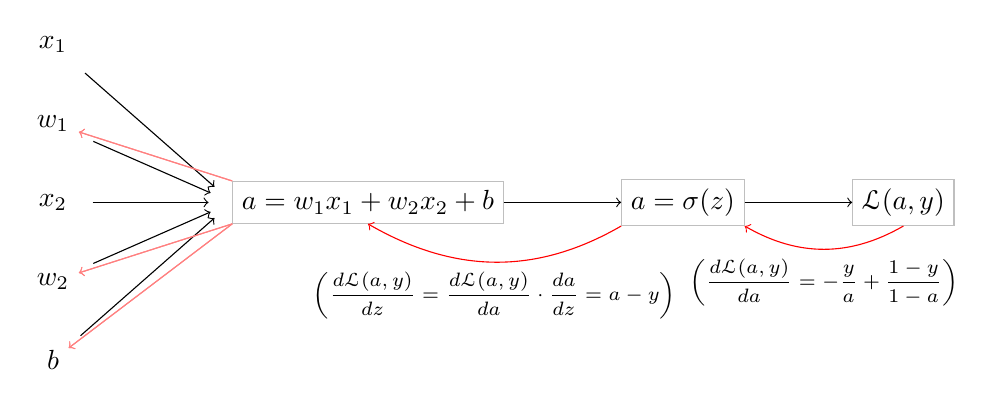
\begin{tikzpicture}
    \node (x1) at (0, 0) {$x_1$}; 
    \node (w1) at (0, -1) {$w_1$};
    \node (x2) at (0,-2) {$x_2$};
    \node (w2) at (0,-3) {$w_2$};
    \node (b) at (0,-4) {$b$};
    \node[rectangle,draw=gray!50] (a) at (4,-2) {$a = w_1 x_1 + w_2 x_2 + b$};
	\node[rectangle,draw=gray!50] (y) at (8,-2) {$a = \sigma(z)$};	
	\node[rectangle,draw=gray!50] (l) at (10.8,-2) {$\L(a,y)$};
    \begin{scope}[every path/.style={shorten <= 0.2cm,shorten >=0.3cm,->}]
       \draw (x1) -- (a.west);
       \draw (w1) -- (a.west); 
       \draw (x2) -- (a.west);
       \draw (w2) -- (a.west);
       \draw (b) -- (a.west);       
    \end{scope}  
    \begin{scope}[every path/.style={->}]
    	\draw (a) -- (y);
       	\draw (y) -- (l);
    \end{scope}
    \begin{scope}[every path/.style={->}]    
       	\draw[red] (l.south) to [out=210, in=330] node [below,black] 
       	{\scriptsize $\bigg( \dfrac{d\L(a,y)}{da}= - \dfrac{y}{a} + \dfrac{1-y}{1-a}\bigg)$} (y.south east) ;
       	\draw[red](y.south west) to [out=210, in=330] node [below,black] 
       	{\scriptsize $\bigg( \dfrac{d\L(a,y)}{dz} = \dfrac{d\L(a,y)}{da} \cdot \dfrac{da}{dz} = a-y \bigg)$} (a.south);
       	\draw[red!50] (a.south west) -- (b);
       	\draw[red!50] (a.north west) -- (w1);
       	\draw[red!50] (a.south west) -- (w2);      	
       
    \end{scope}
    \begin{scope}[every path/.style={->}]    
       	\draw[red!50] (a.south west) -- (b);
       	\draw[red!50] (a.north west) -- (w1);
       	\draw[red!50] (a.south west) -- (w2);
    \end{scope}
\end{tikzpicture}
\end{center}
\end{figure}


See Figure \ref{fig:forwardbackprop} for forward/back. Final step in back prop is how much to change w and b.

\chapter{Neural Network Regularization}
\section{L1 and L2 Regularization}
Given $w \in \R^{n_x}$, $b \in \R$ we want $\min_{w,b} \J(w,b)$
\begin{align}
\J(w,b) &= \dfrac{1}{m} \sum_{i=1}^{m} \L\big( \hat{y}^{(i)}, y^{(i)}) 
	+ \dfrac{\lambda}{2m} \norm{w}^2_2 \textcolor{red}{+ \dfrac{\lambda}{2m} b^2}\\
\text{where } \norm{w}^2_2 &= \sum_{j=1}^{n_x} w_j^2 = w^\intercal w
\end{align}

$\norm{w}^2_2$ is called \textit{L2 Regularization}. The term in red, can be omitted as $w$ is usually a high dimensional parameter vector, but $b$ is just a single number, so almost all params are in $w$ not $b$ so the red term, in practice, likely won't make much of a difference.

\textit{L1 Regularization} is defined as follows
\begin{align}
\dfrac{\lambda}{2m} \sum_{i=1}^{n_x} \lvert w \rvert = \dfrac{\lambda}{2m} \norm{w}_1
\end{align}

$m$ or $2m$ can be used in the denominator, it is just a scaling constant. If you use L1, $w$ will end up being sparse - will have a lot of zeroes - this can help in using less memory, but in practice it is not used much for this. L2 regularization is used much more often.

$\lambda$ is the \textit{regularization parameter} this is usually set using the development set/hold-out cross validation - trying a variety of values to see what does the best, in terms of trading off between doing well in your training set $\dfrac{1}{m} \sum_{i=1}^{m} \L\big( \hat{y}^{(i)}, y^{(i)})$ vs. getting the 2 normal of your parameters,$\dfrac{\lambda}{2m} \norm{w}^2_2$, to be small.

\section{L2 Regularization Within A Neural Net}

\begin{align}
\J(w^{[1]}, b^{[1]}, \ldots, w^{[L]}, b^{[L]}) = 
	\dfrac{1}{m} \sum_{i=1}^{m} \L(\hat{y}^{(i)}, y^{(i)}) 
	+ \dfrac{\lambda}{2m} \sum_{l=1}^{L} \norm{w^{[l]}}^2
\end{align}

$\norm{w^{[l]}}^2$ is the squared norm of matrix $w^{[l]}$, and is defined as

\begin{align}
\norm{w^{[l]}}^2 &= \sum_{i=1}^{n^{[l - 1]}} \sum_{j = 1}^{n^{[l]}}
	\big( w_{ij}^{[l]} \big)^2 \\
	\text{where } w &\in \R^{n^{[l]} \times n^{[l - 1]}}
\end{align}

The shape of $w$, $(n^{[l]}, n^{[l - 1]})$ denotes the number of hidden layers in layer $l$ and $l -1$. Note that the $L2$ norm is called the \textit{Frobenius norm} of a matrix.


\section{How Do We Implement Gradient Descent?}
Compute $dW^{[l]}$ using backward propagation, this would give us $\dfrac{\partial J}{\partial W^{[l]}}$, update $W^{[l]} - \alpha dW^{[l]}$. Now, instead we will add the regularization term to the result of back propagation giving us $dW^{[l]} = \text{ back prop result } + \dfrac{\lambda}{m} W^{[l]}$. 

\begin{align}
W^{[l]} &:= W^{[l]} \lambda \big[ (\text{from back prop}) + \dfrac{\lambda}{m} W^{[l]} \big] \\
	&= W^{[l]} - \dfrac{\alpha \lambda}{m} W^{[l]} - \alpha \text{(from back prop)}
\end{align}

Note that $\dfrac{\partial J}{\partial W^{[l]}} = dW^{[l]}$, also note that $(1- \dfrac{\alpha\lambda}{m}) W^{[l]} = W^{[l]} - \dfrac{\alpha\lambda}{m} W^{[l]}$ so what you are doing when updating $W^{[l]}$ is multiplying it by something slightly less than $1$. It's for these reasons that L2 Regularization is sometimes called \textit{weight decay}.

\section{How Does It Prevent Overfitting?}
To illustrate with layer $l=3$

\[
d3 = np.random.rand
\]

\appendix
\chapter{Basics}
Definitions for some basic notation.
\begin{itemize}
\item $\big[:=\big]$ : update, e.g $x := x + 1$, update $x$ to be $x +1$.
\end{itemize}
\chapter{Notation}
\section{Layers}

\begin{figure}
\caption{Neural Network}
\label{fig:app-neuralnet-1}
\begin{center}
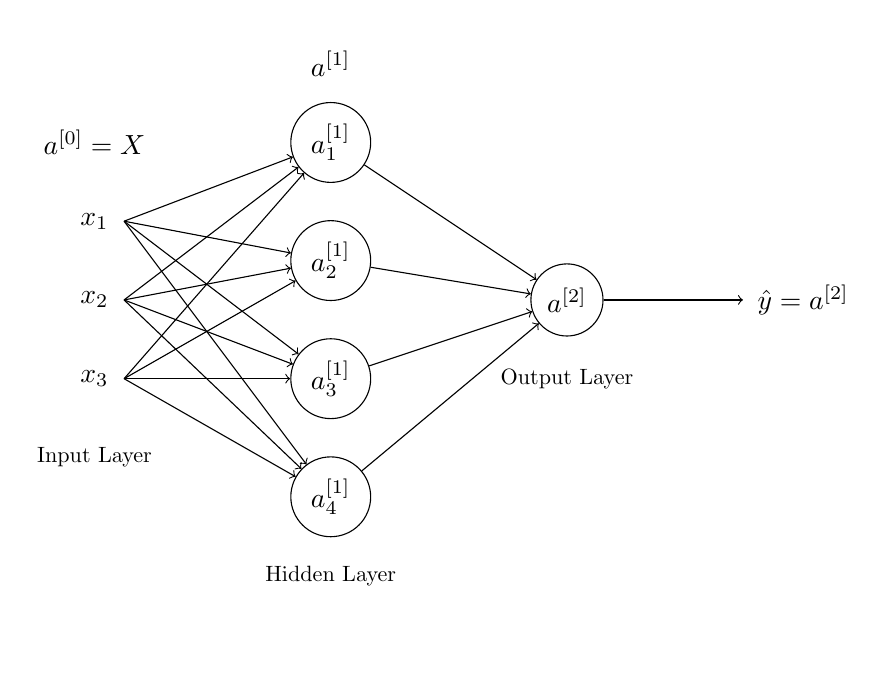
\begin{tikzpicture}
 \begin{scope}[every node/.append style={circle, draw=black}]
 	\node[draw=none] (xnote) at (0, 1) {$a^{[0]} = X$};
    \node[draw=none] (x1) at (0, 0) {$x_1$}; 
    \node[draw=none] (x2) at (0, -1) {$x_2$};
    \node[draw=none] (x3) at (0,-2) {$x_3$};
    \node[draw=none, scale=0.8] (xd) at (0, -3) {Input Layer};

 	\node[draw=none] (hnote) at (3, 2) {$a^{[1]}$};    
    \node (h11) at (3,1) {$a_1^{[1]}$};
    \node (h12) at (3,-0.5) {$a_2^{[1]}$};
    \node (h13) at (3,-2) {$a_3^{[1]}$};
    \node (h14) at (3,-3.5) {$a_4^{[1]}$};
	\node[draw=none, scale=0.8] (hd) at (3,-4.5) {Hidden Layer};
    
    \node (o1) at (6, -1) {$a^{[2]}$};
	\node[draw=none, scale=0.8] (hd) at (6,-2) {Output Layer};
	    
    \node[draw=none] (yhat) at (9, -1) {$\hat{y} = a^{[2]}$};
    \begin{scope}[every path/.style={->}]    
       	\draw (x1.east) -- (h11);
       	\draw (x1.east) -- (h12);
      	\draw (x1.east) -- (h13);
     	\draw (x1.east) -- (h14);
       	
       	\draw (x2.east) -- (h11);
       	\draw (x2.east) -- (h12);
      	\draw (x2.east) -- (h13);
     	\draw (x2.east) -- (h14);
     	
		\draw (x3.east) -- (h11);
      	\draw (x3.east) -- (h12);
      	\draw (x3.east) -- (h13);
     	\draw (x3.east) -- (h14);
     	
     	\draw (h11) -- (o1);
     	\draw (h12) -- (o1);
     	\draw (h13) -- (o1);
     	\draw (h14) -- (o1);
     	
     	\draw (o1) -- (yhat);
     	
    \end{scope}
\end{scope}
\end{tikzpicture}
\end{center}
\end{figure}

Figure \ref{fig:app-neuralnet-1} outlines a 2 layer neural network. The \textit{hidden layer}, $a^{[1]}$ has four dimensions - as we have four hidden units in the hidden layer - vectorizing this we get

\[
a^{[1]} =  \begin{bmatrix}
	a^{[1]}_1 \\
	a^{[1]}_2 \\
	a^{[1]}_3 \\	
	a^{[1]}_4 \\
\end{bmatrix}
\]

In general for a hidden layer $l$ of $n$ components we would get

\[
a^{[l]} =  \begin{bmatrix}
	a^{[l]}_1 \\
	a^{[l]}_2 \\
	\vdots \\
	a^{[l]}_n \\
\end{bmatrix}
\]

The hidden layer and output layers will have parameters associated with them - $W$ and $b$. In this case, for the hidden layer we have $W \in \R^{4 \times 3}$ and $b \in \R^{4 \times 1}$ and for the output layer $W \in \R^{1 \times 4}$ and $b \in \R^{1 \times 1}$.


% End of book

\pagestyle{headings}
\pagenumbering{arabic}

\include{ch1}
\include{ch2}

\begin{thebibliography}{99}
  \addcontentsline{toc}{chapter}{Bibliography}
\bibitem{lamport} L. Lamport. {\bf \LaTeX \ A Document Preparation System}
Addison-Wesley, California 1986.
\end{thebibliography}

\include{index}
 \addcontentsline{toc}{chapter}{Index}
\end{document}
